\section{\chameleon{} Prototype and RVSI Protocol}

% System Design of \chameleon{}

%%%%%%%%%%%%%%%
\begin{frame}{}
  \begin{center}
    \chameleon{} prototype: \\[10pt]
    A prototype \textbf{partitioned} \textbf{replicated} \\[6pt]
    distributed transactional \textbf{key-value} store
  \end{center}
\end{frame}
%%%%%%%%%%%%%%%

%%%%%%%%%%%%%%%
\begin{frame}{}
  \begin{center}
    Classic \textbf{key-value} data model \\[4pt]
      Key: (row key, column key)
  \end{center}
\end{frame}
%%%%%%%%%%%%%%%

%%%%%%%%%%%%%%%
\begin{frame}{}
  % \fignocaption{width = 0.70\textwidth}{figs/chameleon-arch.pdf}
  \begin{center}
    \resizebox{0.70\textwidth}{!}{%        File: chameleon-arch.tex
%     Created: Mon Jan 04 08:00 PM 2016 C
% Last Change: Mon Jan 04 08:00 PM 2016 C
% 	    Used in Beamer

\begin{tikzpicture}[connection/.style = {>=Stealth, <->, brown, dashed, line width = 3pt}]
  % background: china map
  \node (china-map) [opacity = 0.20] {
\includegraphics[scale = 0.40]{figs/china-outline-blue.png}};

  % partition-left, partition-right, partition-below
  \uncover<2->{
    \node (partition-left) [] at (-6.5, 1) {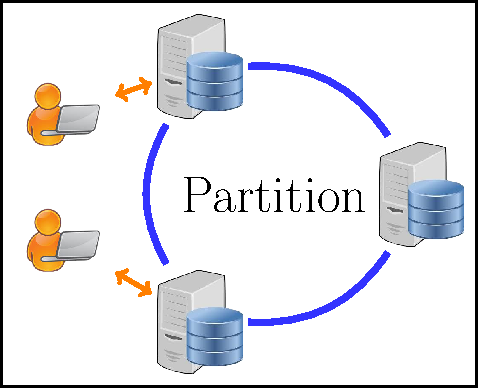
\includegraphics[scale = 0.80]{figs/partition.pdf}}; 
  }
  \uncover<3->{
    \node (partition-right) [] at (6, 3.5) {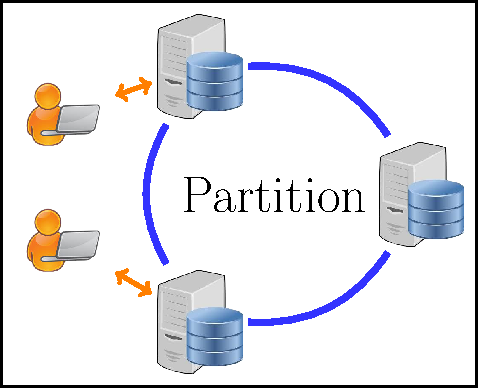
\includegraphics[scale = 0.80]{figs/partition.pdf}}; 
    \node (partition-below) [] at (1.5, -5) {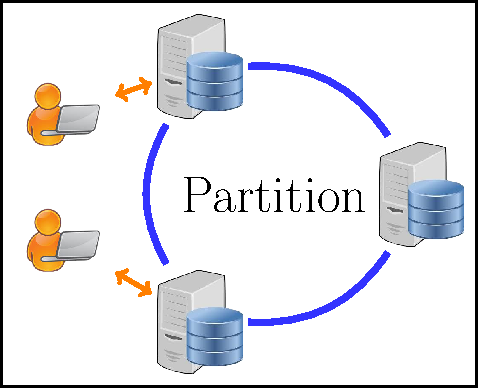
\includegraphics[scale = 0.80]{figs/partition.pdf}}; 

    % connections among partitions
    \draw [connection] (partition-left) to (partition-right); 
    \draw [connection] (partition-right) to (partition-below);
    \draw [connection] (partition-below) to (partition-left);

    % replication 
    \node (replication) [font = \Huge, align = center] at (0.5, 0.0) {\textbf{Wide-area}\\[3pt]\textbf{Replication}};
  }

  \uncover<4->{
    % master-slave for one partition
    \begin{scope}[circled/.style = {draw, circle, dash pattern = on 10pt off 5pt, cyan, line width = 2pt, outer sep = 5pt, minimum size = 2.0cm}, 
      conn/.style = {dash pattern = on 15pt off 8pt, cyan, line width = 2pt}]
    \node (ms-left) [circled] at (-4., 1) {};
    \node (ms-right) [circled] at (5.5, 1.7) {};
    \node (ms-below) [circled] at (4., -5.0) {};

    \node (master-slave) [below right = 1.5cm and -1.5cm of partition-right] {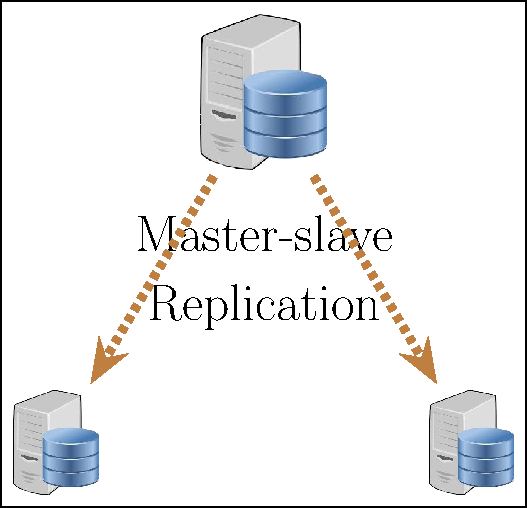
\includegraphics[scale = 0.80]{figs/master-slave.pdf}};
    \draw [conn] (ms-left) to (master-slave);
    \draw [conn] (ms-right) to (master-slave);
    \draw [conn] (ms-below) to (master-slave);
    \end{scope}
  }
\end{tikzpicture}
}
  \end{center}

  \begin{center}
    \only<2>{Keys are \textbf{partitioned} within a single datacenter.}
    \only<3-4>{Each key is \textbf{replicated} across datacenters} \only<4>{in a \textbf{master-slave} manner.}
    \only<5>{Transactions are first executed and committed on the \textbf{masters},\\
      and are then asynchronously propagated to \textbf{slaves}.}
  \end{center}
\end{frame}
%%%%%%%%%%%%%%%

%%%%%%%%%%%%%%%
\begin{frame}{}
  \only<1-3, 5->{\fignocaption{width = 0.50\textwidth}{figs/chameleon-framework.pdf}}

  \begin{center}
    \only<2>{\blue{1.} Partitioned replicated transactional key-value store}
    \only<3>{\blue{2.} Client library}
    \only<5>{\blue{3.} \rvsi{} protocol: \rvsims{} + \rvsimp{}}
  \end{center}

  \only<4>{
    Code snippet for writing \rvsi{} transactions: \\[8pt]
    \begin{lstlisting}[
  language = Java,
  basicstyle = \ttfamily\footnotesize,
  showstringspaces = false,
  keywordstyle = \color{blue}\bfseries,
  commentstyle = \color{teal},
  stringstyle = \bfseries,
  upquote = true,
  frame = box,
  breaklines = true,
  linewidth = 0.85\textwidth
]
  // Initialize keys (ck, ck1, and ck2) here
  ITx tx = new RVSITx(/** context **/);

  tx.begin();

  // Read and write
  ITsCell tsCell = tx.read(ck);
  ITsCell tsCell1 = tx.read(ck1);
  tx.write(ck1, new Cell("R1C1"));
  ITsCell tsCell2 = tx.read(ck2);

  // Specify RVSI specs. (e.g., SVSpec)
  RVSISpec sv = new SVSpec();
  sv.addSpec({ck, ck1, ck2}, 2);
  tx.collectRVSISpec(sv);

  boolean committed = tx.end();
\end{lstlisting}

  }
\end{frame}
%%%%%%%%%%%%%%%


% the RVSI-MS protocol
%%%%%%%%%%%%%%%
\begin{frame}{}
  \centerline{\textbf{\rvsims{}}: RVSI protocol for master-slave replication}

  \vspace{1.0cm}
  In terms of \emph{event} generation and handling:
  \begin{description}
    \item[Clients:] \ebegin, \eread, \ewrite, \eend%
    \item[Master:] \estart, \ecommit, \esend%
    \item[Slaves:] \ereceive%
  \end{description}
\end{frame}
%%%%%%%%%%%%%%%

%%%%%%%%%%%%%%%
\begin{frame}{}
  TikZ overlay for \rvsims{}
\end{frame}
%%%%%%%%%%%%%%%

%%%%%%%%%%%%%%%
\begin{frame}{}
  Calculating version constraints:
\end{frame}
%%%%%%%%%%%%%%%

% the RVSI-MP protocol
%%%%%%%%%%%%%%%
\begin{frame}{}
  \begin{center}
    Distributed transactions spanning multiple masters need to be committed atomically.

    \pause
    Using the two-phase commit (2PC) protocol.
  \end{center}
\end{frame}
%%%%%%%%%%%%%%%

%%%%%%%%%%%%%%%
\begin{frame}{}
  Assumes a timestamp oracle:
  \begin{description}
    \item[Clients:] 
    \item[Masters:]
  \end{description}
\end{frame}
%%%%%%%%%%%%%%%

%%%%%%%%%%%%%%%
\begin{frame}{}
  \rvsi{} version constraints in 2PC protocol:
  \begin{description}
    \item[$\konebv$:]
    \item[$\ktwofv$:]
    \item[$\kthreesv$:]
  \end{description}
\end{frame}
%%%%%%%%%%%%%%%

%%%%%%%%%%%%%%%
\begin{frame}{}
  \begin{figure}[t]
    \begin{algorithm}[H]
  \caption{\rvsims{}: RVSI Protocol for Replication (for Executing Transaction $T$).}
  \label{alg:rvsims}
  \begin{algorithmic}[1]
    %%%%%%%%%%%%%%%%%%%%%%%%%%%%%%%%%%%%%%%% For clients %%%%%%%%%%%%%%%%%%%%%%%%%%%%%%%%%%%%%%%%
    \Statex \textbf{\textit{Client-side methods:}}
    \hStatex

    \Procedure{begin}{\null}
    \State $T.\attr{sts}$ $\gets$ \algkeyword{rpc-call} \Call{start}{\null} at master 
    $\master$   \label{line:call-start}
    \EndProcedure

    \Procedure{read}{$x$}
      \State $x.\attr{ver}$ $\gets$ \algkeyword{rpc-call} \Call{read}{$x$} at any site
    \EndProcedure

    \Procedure{write}{$x, v$}
      \State add $(x, v)$ to $T.\attr{writes}$ \label{line:write-at-client}
    \EndProcedure

    \Procedure{end}{$T$}
    \State $T.\attr{vc}$ $\gets$ \Call{add-vc}{\null} \label{line:call-add-vc}
    \State $c/a$ $\gets$ \algkeyword{rpc-call} \Call{commit}{$T.\attr{writes}, 
    T.\attr{vc}$} at $\master$ \label{line:call-commit}
    \EndProcedure

    \Statex \hrulefill

    %%%%%%%%%%%%%%%%%%%%%%%%%%%%%%%%%%%%%%%% For master %%%%%%%%%%%%%%%%%%%%%%%%%%%%%%%%%%%%%%%%
    \Statex \textbf{\textit{Master-side data structures and methods:}}
    \Statex $\master$.\attr{ts}: for start-timestamps and commit-timestamps
    \Statex $\set{x.\attr{ver} = (x.\attr{ts}, x.\attr{ord}, x.\attr{val})}$: set of versions of $x$
    \hStatex

    \Procedure{start}{\null}
    \State \Return ++$\master.\attr{ts}$
    \EndProcedure
    
    \Procedure{read}{$x$}
      \State \Return the latest $x.\attr{ver}$ installed \label{line:read-at-master}
    \EndProcedure

    \Procedure{commit}{$T.\attr{writes}, T.\attr{vc}$}
    \If{\Call{check-vc}{$T.\attr{vc}$} \&\& write-conflict freedom}   
    \label{line:call-check-vc}
      \State $T.\attr{cts}$ $\gets$ ++$\master.\attr{ts}$ 

      \lComment{apply $T.\attr{writes}$ locally and propagate it} 
      \State $T.\textrm{\it upvers} = \emptyset$  \mComment{collect updated versions}  
      \label{line:commit-updates}
      \For{$(x,v) \in T.\attr{writes}$}    
      \State $x.\attr{new-ver} \gets (T.\attr{cts}, \textrm{++}x.\attr{ord}, v)$
      \State add $x.\attr{new-ver}$ to $\set{x.\attr{ver}}$ and $T.\textrm{\it upvers}$
      \EndFor 
      \State \algkeyword{broadcast} \msg{PROP}{T.\textrm{\it upvers}} to slaves 
      \label{line:commit-prop}
      % \lendComment{apply $T.\attr{writes}$ locally and propagate it} 

      \State \Return $c$ denoting ``committed''
    \EndIf
    \State \Return $a$ denoting ``aborted''
    \EndProcedure

    \Statex \hrulefill

    %%%%%%%%%%%%%%%%%%%%%%%%%%%%%%%%%%%%%%%% For slaves %%%%%%%%%%%%%%%%%%%%%%%%%%%%%%%%%%%%%%%%
    \Statex \textbf{\textit{Slave-side data structures and methods:}}
    \Statex $x.\attr{ver} = (x.\attr{ts}, x.\attr{ord}, x.\attr{val})$: the latest version of $x$
    \hStatex

    \Procedure{read}{$x$}
    \State \Return $x.\attr{ver}$
    \EndProcedure

    \algrenewcommand\algorithmicprocedure{\textbf{upon}}
    \Procedure{received}{\msg{PROP}{T.\textrm{\it upvers}}} \label{line:received}
    \For{$\left(x.\attr{ver}' = (x.\attr{ts}', x.\attr{ord}', x.\attr{val}')\right) \in 
    T.\textrm{\it upvers}$}
      \If{$x.\attr{ord}' > x.\attr{ord}$}  
      \State $x.\attr{ver} \gets x.\attr{ver}'$
      \EndIf
    \EndFor
    \EndProcedure
  \end{algorithmic}
\end{algorithm}

    % \resizebox{0.90\linewidth}{!}{\begin{algorithm}[H]
  \caption{\rvsims{}: RVSI Protocol for Replication (for Executing Transaction $T$).}
  \label{alg:rvsims}
  \begin{algorithmic}[1]
    %%%%%%%%%%%%%%%%%%%%%%%%%%%%%%%%%%%%%%%% For clients %%%%%%%%%%%%%%%%%%%%%%%%%%%%%%%%%%%%%%%%
    \Statex \textbf{\textit{Client-side methods:}}
    \hStatex

    \Procedure{begin}{\null}
    \State $T.\attr{sts}$ $\gets$ \algkeyword{rpc-call} \Call{start}{\null} at master 
    $\master$   \label{line:call-start}
    \EndProcedure

    \Procedure{read}{$x$}
      \State $x.\attr{ver}$ $\gets$ \algkeyword{rpc-call} \Call{read}{$x$} at any site
    \EndProcedure

    \Procedure{write}{$x, v$}
      \State add $(x, v)$ to $T.\attr{writes}$ \label{line:write-at-client}
    \EndProcedure

    \Procedure{end}{$T$}
    \State $T.\attr{vc}$ $\gets$ \Call{add-vc}{\null} \label{line:call-add-vc}
    \State $c/a$ $\gets$ \algkeyword{rpc-call} \Call{commit}{$T.\attr{writes}, 
    T.\attr{vc}$} at $\master$ \label{line:call-commit}
    \EndProcedure

    \Statex \hrulefill

    %%%%%%%%%%%%%%%%%%%%%%%%%%%%%%%%%%%%%%%% For master %%%%%%%%%%%%%%%%%%%%%%%%%%%%%%%%%%%%%%%%
    \Statex \textbf{\textit{Master-side data structures and methods:}}
    \Statex $\master$.\attr{ts}: for start-timestamps and commit-timestamps
    \Statex $\set{x.\attr{ver} = (x.\attr{ts}, x.\attr{ord}, x.\attr{val})}$: set of versions of $x$
    \hStatex

    \Procedure{start}{\null}
    \State \Return ++$\master.\attr{ts}$
    \EndProcedure
    
    \Procedure{read}{$x$}
      \State \Return the latest $x.\attr{ver}$ installed \label{line:read-at-master}
    \EndProcedure

    \Procedure{commit}{$T.\attr{writes}, T.\attr{vc}$}
    \If{\Call{check-vc}{$T.\attr{vc}$} \&\& write-conflict freedom}   
    \label{line:call-check-vc}
      \State $T.\attr{cts}$ $\gets$ ++$\master.\attr{ts}$ 

      \lComment{apply $T.\attr{writes}$ locally and propagate it} 
      \State $T.\textrm{\it upvers} = \emptyset$  \mComment{collect updated versions}  
      \label{line:commit-updates}
      \For{$(x,v) \in T.\attr{writes}$}    
      \State $x.\attr{new-ver} \gets (T.\attr{cts}, \textrm{++}x.\attr{ord}, v)$
      \State add $x.\attr{new-ver}$ to $\set{x.\attr{ver}}$ and $T.\textrm{\it upvers}$
      \EndFor 
      \State \algkeyword{broadcast} \msg{PROP}{T.\textrm{\it upvers}} to slaves 
      \label{line:commit-prop}
      % \lendComment{apply $T.\attr{writes}$ locally and propagate it} 

      \State \Return $c$ denoting ``committed''
    \EndIf
    \State \Return $a$ denoting ``aborted''
    \EndProcedure

    \Statex \hrulefill

    %%%%%%%%%%%%%%%%%%%%%%%%%%%%%%%%%%%%%%%% For slaves %%%%%%%%%%%%%%%%%%%%%%%%%%%%%%%%%%%%%%%%
    \Statex \textbf{\textit{Slave-side data structures and methods:}}
    \Statex $x.\attr{ver} = (x.\attr{ts}, x.\attr{ord}, x.\attr{val})$: the latest version of $x$
    \hStatex

    \Procedure{read}{$x$}
    \State \Return $x.\attr{ver}$
    \EndProcedure

    \algrenewcommand\algorithmicprocedure{\textbf{upon}}
    \Procedure{received}{\msg{PROP}{T.\textrm{\it upvers}}} \label{line:received}
    \For{$\left(x.\attr{ver}' = (x.\attr{ts}', x.\attr{ord}', x.\attr{val}')\right) \in 
    T.\textrm{\it upvers}$}
      \If{$x.\attr{ord}' > x.\attr{ord}$}  
      \State $x.\attr{ver} \gets x.\attr{ver}'$
      \EndIf
    \EndFor
    \EndProcedure
  \end{algorithmic}
\end{algorithm}
}
  \end{figure}
\end{frame}
%%%%%%%%%%%%%%%

%%%%%%%%%%%%%%%
\begin{frame}{}
  \begin{figure}[t]
    %%%%% file: alg-rvsi-partition.tex
%%%%% description: protocol for distributed transactions across multiple partitions; using 2PC 

\begin{algorithm}[H]
  \caption{\rvsimp{}: \rvsi{} Protocol for Partition (for Executing Transaction $T$).} % (\algnamefont{RVSI-MP})}
  \label{alg:alg-rvsi-partition}
  \begin{algorithmic}[1]
    %%%%%%%%%%%%%%%%%%%%%%%%%%%%%%%%%%%%%%%% For clients %%%%%%%%%%%%%%%%%%%%%%%%%%%%%%%%%%%%%%%%
    \Statex \textbf{\textit{Client-side methods:}}
    \hStatex

    \Procedure{begin}{\null}
	\State \Return \algkeyword{rpc-call} \Call{getTS}{\null} at $\timeoracle{}$
		\label{line:rvsimp-client-call-getts}
    \EndProcedure

	\Procedure{end}{\null}	\label{line:rvsimp-call-end}
      \State $T.\attr{vc}$ $\gets$ \Call{add-vc}{\null} \label{line:rvsimp-call-add-vc}
      \State $c/a$ $\gets$ \algkeyword{rpc-call} \Call{c-commit}{$T.\attr{writes}, T.\attr{vc}$} 
      at $\coordinator$ \label{line:rvsimp-call-commit}
    \EndProcedure

    \Statex \hrulefill
    %%%%%%%%%%%%%%%%%%%% For Timestamp Oracle %%%%%%%%%%%%%%%%%%%%
    \Statex \textbf{\textit{Timestamp oracle methods:}}
    \hStatex
	\Statex \tots{}: for start-timestamps and commit-timestamps

	\Procedure{getTS}{\null}	\label{line:rvsimp-getts}
	  \State \Return ++\tots{}
	\EndProcedure

    \Statex \hrulefill
    %%%%%%%%%%%%%%%%%%%%%%%%%%%%%%%%%%%%%%%% For coordinator %%%%%%%%%%%%%%%%%%%%%%%%%%%%%%%%%%%%%%%%
    \Statex \textbf{\textit{Coordinator-side data structures and methods:}}
    \Statex The coordinator $\coordinator$ executes the 2PC protocol with masters $\master$ involved in $T$.
    \hStatex

	\Procedure{c-commit}{$T.\attr{writes}, T.\attr{vc}$}	\label{line:rvsimp-ccommit}
	\State split $T.\attr{writes}$ and $\tvc{T}$ with the data partitioning strategy	
	  \label{line:rvsimp-partition}
	  \hStatex

      \lComment{the prepare phase:}
	  \State \algkeyword{rpc-call} \Call{prepare}{$T.\attr{writes}, T.\attr{vc}$} at each $\master$
		\label{line:rvsimp-call-prepare}

      \lComment{the commit phase:}
      \If{all \Call{prepare}{$T.\attr{writes}, T.\attr{vc}$} return \textsl{true}}
		\label{line:rvsimp-prepare-all-true}
	  \State $T.\attr{cts} \gets$ \algkeyword{rpc-call} 
		\Call{getTS}{\null} at $\timeoracle$
		  \label{line:rvsimp-coord-call-getts}
		\State \algkeyword{rpc-call} \Call{commit}{$T.\attr{cts}, T.\attr{writes}$} at each $\master$
		  \label{line:rvsimp-coord-call-commit}
		%   \lComment{early commit notification~\cite{binnig:vldb14}}
        % \State \Return $c$ denoting ``commited''    
      \Else
        \State \algkeyword{rpc-call} \Call{abort}{\null} at each $\master$
		  \label{line:rvsimp-coord-call-abort}
        \State \Return $a$ denoting ``aborted''
      \EndIf

	  \If{all \Call{commit}{$T.\attr{cts}, T.\attr{writes}$} return \textsl{true}}
        \State \Return $c$ denoting ``committed''
	  \Else
		\State \Return $a$ denoting ``aborted''
      \EndIf
    \EndProcedure
    
    \Statex \hrulefill
    %%%%%%%%%%%%%%%%%%%%%%%%%%%%%%%%%%%%%%%% For masters %%%%%%%%%%%%%%%%%%%%%%%%%%%%%%%%%%%%%%%%
    \Statex \textbf{\textit{Master-side methods:}}
    \hStatex

    \Procedure{prepare}{$T.\attr{writes}, T.\attr{vc}$} \label{line:rvsimp-prepare}
      \State \Return \Call{check-vc}{$T.\attr{vc}$} \&\& write-conflict freedom
		\label{line:rvsimp-check-in-prepare}
    \EndProcedure

	\Procedure{commit}{$T.\attr{cts}, T.\attr{writes}$}	\label{line:rvsimp-commit}
	  \lComment{apply $T.\attr{writes}$ locally and propagate it} 
		\label{line:rvsimp-apply-in-commit}
    \EndProcedure

	\Procedure{abort}{\null}  \label{line:rvsimp-abort}
	\lComment{abort}
    \EndProcedure
  \end{algorithmic}
\end{algorithm}

  \end{figure}
\end{frame}
%%%%%%%%%%%%%%%

%%%%%%%%%%%%%%%
\begin{frame}{}
\end{frame}
%%%%%%%%%%%%%%%
